\documentclass[letterpaper,11pt]{article}

\usepackage{afterpage}
\usepackage{amsmath}
\usepackage{amssymb}
\usepackage{bm}
\usepackage[hmargin=1.25in,vmargin=1in]{geometry}
\usepackage{booktabs}
\usepackage{graphicx}
\usepackage{hyperref}
\usepackage{lmodern}
\usepackage{microtype}
\usepackage{pdflscape}
\usepackage{subcaption}

\title{Coursework 7: STAT 570}
\author{Philip Pham}
\date{\today}

\begin{document}
\maketitle
\begin{enumerate}
\item Create a binary variable $Z_i$, with $Z_i = 0$ corresponding to
  $Y_i \in \{0,1\}$ and $Z_i = 1$ corresponding to $Y_i \in \{2,3\}$. Let
  $q\left(x_i\right) = \mathbb{P}(Z_i = 1 \mid x_i)$, with
  $\mathbf{x}_i = \begin{pmatrix} 1 & x_{1i} & x_{2i}
  \end{pmatrix}^\intercal$, represent the probability of mental impairment being
  \emph{Moderate} or \emph{Impaired}, given covariates $\mathbf{x}_i$,
  $i = 1,\ldots,n = 40$.  Provide a single plot that shows the association
  between $q\left(x_i\right)$ and $x_{1i}$ and $x_{2i}$, on a response scale
  you feel is appropriate. Comment on the plot.

  \begin{figure}[h]
    \centering
    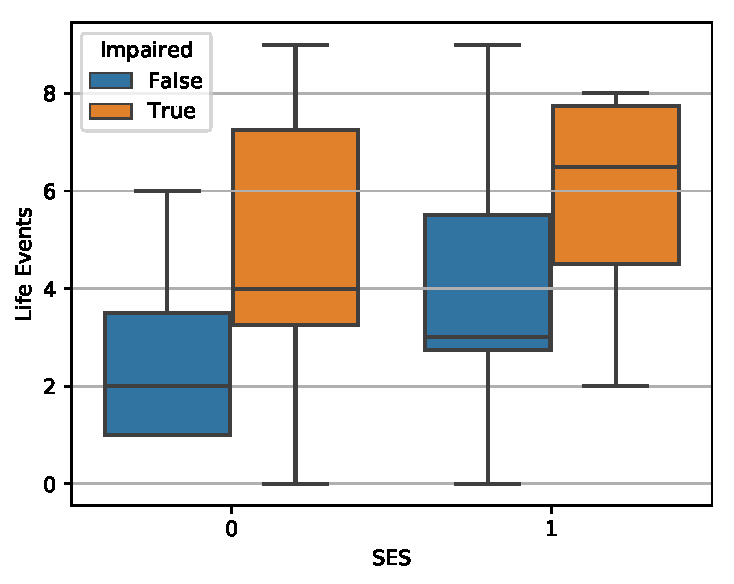
\includegraphics{p1_descriptive.pdf}
    \caption{Orange denotes $Z_i = 1$ and blue denotes $Z_i = 0$.}
    \label{fig:p1_descriptive}
  \end{figure}
  
  \begin{description}
  \item[Solution:] See Figure \ref{fig:p1_descriptive}. Conditioned on SES,
    those that are impaired ($Z_i = 1$) have a greater number of life events on
    average.
  \end{description}
\item Suppose $Z_i \mid q_i \sim \operatorname{Binomial}\left(1, q_i\right)$
  independently for $i = 1,\ldots, n = 40$, where $q_i =
  q\left(x_i\right)$. Consider the logistic regression model,
  \begin{equation}
    q\left(x_i\right) = \log\left(
      \frac{q\left(\mathbf{x}_i\right)}{1 - q\left(\mathbf{x}_i\right)}
    \right)
    =
    \mathbf{x}_i^\intercal \bm{\gamma}
    = \gamma_0 + \gamma_1 x_{1i} + \gamma_2 x_{2i},
    \label{eqn:p2_model}
  \end{equation}  
  where $\bm{\gamma} = \begin{pmatrix}\gamma_0 & \gamma_1 & \gamma_2
  \end{pmatrix}^\intercal$. Write down the log-likelihood
  $l\left(\bm{\gamma}\right)$ for the sample $z_i$, $i = 1,\ldots, n$.

  \begin{description}
  \item[Solution:] Solving for $q\left(\mathbf{x}_i\right)$ in Equation
    \ref{eqn:p2_model}, we find
    \begin{equation}
      q\left(\mathbf{x}_i\right)
      = \frac{\exp\left(\mathbf{x}_i^\intercal \bm{\gamma}\right)}
      {1 + \exp\left(\mathbf{x}_i^\intercal \bm{\gamma}\right)}
      = \frac{1}
      {1 + \exp\left(-\mathbf{x}_i^\intercal \bm{\gamma}\right)}.
      \label{eqn:p2_qi}
    \end{equation}

    The likelihood function is
    $L\left( \bm{\gamma} \right) = \prod_{i=1}^n
    \left(q\left(\mathbf{x}_i\right)\right)^{z_i} \left(1 -
      q\left(\mathbf{x}_i\right)\right)^{1 - z_i}$, so the log-likelihood
    function becomes
    \begin{align}
      l\left(\bm{\gamma}\right)
      &= \log L\left( \bm{\gamma} \right)
        = \sum_{i=1}^n \left(
        z_i \log q\left(\mathbf{x}_i\right)
        +
        \left(1 - z_i \right) \log\left(1 - q\left(\mathbf{x}_i\right)\right)
        \right)
        \label{eqn:p2_log_likelihood}\\
      &= \sum_{i=1}^n\left(
        z_i\log\frac{q\left(\mathbf{x}_i\right)}{1 -q\left(\mathbf{x}_i\right)}
        + \log\left(1 -q\left(\mathbf{x}_i\right)\right)
        \right) \nonumber\\
      &= \sum_{i=1}^n
        \left(
        z_i\mathbf{x}_i^\intercal\bm{\gamma} +
        \log\frac{1}{1 + \exp\left(\mathbf{x}_i^\intercal\bm{\gamma}\right)}
        \right)
        = \sum_{i=1}^n
        -\log\left(
        1 + \exp\left(\left(1 - 2z_i\right)\mathbf{x}_i^\intercal\bm{\gamma}\right)
        \right). \nonumber
    \end{align}
  \end{description}
\item Fit the model described in the previous part, and give confidence
  intervals for the odds ratios.

  Carefully interpret these odds ratios.

  \begin{table}[!h]
    \centering
    \begin{tabular}{lrrrr}
\toprule
{} &  Estimate &  Standard error &  95\% CI lower bound &  95\% CI upper bound \\
\midrule
$\gamma_0$ & -0.925065 &        0.723346 &            -2.342797 &             0.492666 \\
$\gamma_1$ & -1.629731 &        0.780849 &            -3.160167 &            -0.099296 \\
$\gamma_2$ &  0.309899 &        0.147920 &             0.019980 &             0.599818 \\
\bottomrule
\end{tabular}

    \caption{Estimates and confidence intervals for $\hat{\bm\gamma}$ using
      maximum likelihood estimation.}
    \label{tab:p3_gamma_hat}
  \end{table}
  
  \begin{description}
  \item[Solution:] Taking the derivative of Equation
    \ref{eqn:p2_log_likelihood}, we have the score function:

    \begin{align}
      S\left(\bm\gamma\right)
      = \nabla^\intercal l\left(\bm\gamma\right)
      &= \sum_{i=1}^n \frac{2z_i - 1}{1 + \exp\left(
        \left(1 - 2z_i\right)\mathbf{x}_i^\intercal\bm{\gamma}
        \right)}\exp\left(
        \left(1 - 2z_i\right)\mathbf{x}_i^\intercal\bm{\gamma}
        \right)\mathbf{x}_i.
        \nonumber\\
      &= \sum_{i=1}^n \frac{2z_i - 1}{1 + \exp\left(
        \left(2z_i - 1\right)\mathbf{x}_i^\intercal\bm{\gamma}
        \right)}\mathbf{x}_i \nonumber\\
      &= X^\intercal\left(
        \mathbf{z} - \mathbf{q}\left(X\right)
        \right),
    \label{eqn:p3_score_function}
    \end{align}
    where
    $\mathbf{z} = \begin{pmatrix}z_1 & z_2 & \cdots & z_n\end{pmatrix}^\intercal$ and
    $\mathbf{q}\left(X\right) = \begin{pmatrix}q_1 & q_2 &
      \cdots & q_n\end{pmatrix}^\intercal$.
    
    From Equation \ref{eqn:p3_score_function}, we have the Fisher information
    matrix:
    \begin{align}
      I_n\left(\bm\gamma\right)
      &= \operatorname{var}\left(S\left(\bm\gamma\right) \mid \bm\gamma\right)
        = \mathbb{E}\left[
        S\left(\bm\gamma\right)
        S\left(\bm\gamma\right)^\intercal
        \mid \bm\gamma
        \right] \nonumber\\
      &= \mathbb{E}\left[
        X^\intercal\left(
        \mathbf{z} - \mathbf{q}\left(X\right)
        \right)
        \left(
        \mathbf{z} - \mathbf{q}\left(X\right)
        \right)^\intercal
        X \mid \bm\gamma
        \right] \nonumber \\
      &= X^\intercal\mathbb{E}\left[
        \left(
        \mathbf{z} - \mathbf{q}\left(X\right)
        \right)
        \left(
        \mathbf{z} - \mathbf{q}\left(X\right)
        \right)^\intercal
        \mid \bm\gamma
        \right]X \nonumber\\
      &= \sum_{i=1}^n 
        q\left(\mathbf{x}_i\right)
        \left(1 - q\left(\mathbf{x}_i\right)\right)
        \mathbf{x}_i\mathbf{x}_i^\intercal
        =
        \sum_{i=1}^n
        \frac{1}{2 + \exp\left(
        -\mathbf{x}_i^\intercal \bm\gamma
        \right) + \exp\left(
        \mathbf{x}_i^\intercal \bm\gamma
        \right)}
        \mathbf{x}_i\mathbf{x}_i^\intercal
        ,
        \label{eqn:p3_fisher_information}
    \end{align}
    where we have used independence of the observations and variance of the
    binomial distribution to get the last line.

    We solve Equation \ref{eqn:p3_score_function},
    $S\left(\hat{\bm{\gamma}}\right) = \mathbf{0}$, to get an estimate for
    $\bm\gamma$. Using Equation \ref{eqn:p3_fisher_information}, we have that
    \begin{equation}
      \hat{\bm\gamma}
      \xrightarrow{\mathcal{D}}
      \mathcal{N}\left(
        \gamma,
        I_n^{-1}\left(\hat{\bm\gamma}\right)
      \right),
      \label{eqn:p3_gamma_hat_dist}
    \end{equation}
    that is, $\hat{\bm\gamma}$ is asymptotically normal.

    Using Equation \ref{eqn:p3_gamma_hat_dist}, we obtain the estimates and
    intervals in Table \ref{tab:p3_gamma_hat}.

    The predicted log odds ratio given some $\mathbf{x}_i$ is
    \begin{equation}
      \hat\theta_i = \mathbf{x}_i^\intercal\hat{\bm\gamma},
      \label{eqn:p3_prediction}
    \end{equation}
    which will have variance
    \begin{equation}
      \operatorname{var}\left(\hat\theta_i\right)
      = \mathbf{x}_i^\intercal\operatorname{var}\left(\hat{\bm\gamma}\right)
      \mathbf{x}_i
      \approx \mathbf{x}_i^\intercal I_n^{-1}\left(\hat{\bm\gamma}\right)
      \mathbf{x}_i,
      \label{eqn:p3_prediction_variance}
    \end{equation}
    using Equation \ref{eqn:p3_gamma_hat_dist}.

    From Equation \ref{eqn:p3_prediction_variance}, we can compute confidence
    intervals for the log odds ratio and exponentiate to get confidence
    intervals for the odds ratio since $\log$ is a monotonic
    transformation. Doing so results in the estimates in Table
    \ref{tab:p3_odds_ratios}.

    The odds ratio is how much more likely one is to have \texttt{Moderate} or
    \texttt{Impaired} mental impairment. Exponentiating Equation
    \ref{eqn:p3_prediction}, we have
    \begin{equation}
      \exp\left(\theta_i\right) =
      \exp\left(\gamma_0\right)
      \exp\left(\gamma_1x_{1i}\right)
      \exp\left(\gamma_2x_{2i}\right).
    \end{equation}
    
    $\exp\left(\gamma_0\right)$ is the expected odds ratio for a subject with
    $0$ SES and no life events. $\exp\left(\gamma_1\right)$ is the expected odds
    ratio between a subject with SES 1 and SES 0. $\exp\left(\gamma_2\right)$ is
    the expected odds ratio for a subject with an additional life event.
  \end{description}
  \begin{table}
    \scriptsize
    \centering
    \begin{tabular}{llrrrr}
\toprule
  &   &  Count &  Estimate &  95\% CI lower bound &  95\% CI upper bound \\
SES & Life Events &        &           &                     &                     \\
\midrule
0 & 0 &      1 &  0.396506 &            0.096059 &            1.636675 \\
  & 1 &      3 &  0.540551 &            0.158334 &            1.845440 \\
  & 2 &      2 &  0.736926 &            0.249432 &            2.177188 \\
  & 3 &      3 &  1.004642 &            0.368208 &            2.741129 \\
  & 4 &      3 &  1.369616 &            0.501460 &            3.740769 \\
  & 5 &      2 &  1.867180 &            0.630203 &            5.532120 \\
  & 6 &      1 &  2.545502 &            0.742501 &            8.726699 \\
  & 8 &      1 &  4.730948 &            0.915136 &           24.457420 \\
  & 9 &      2 &  6.449640 &            0.982321 &           42.346488 \\
1 & 0 &      1 &  0.077708 &            0.011740 &            0.514377 \\
  & 1 &      2 &  0.105938 &            0.020316 &            0.552412 \\
  & 2 &      2 &  0.144424 &            0.034495 &            0.604687 \\
  & 3 &      5 &  0.196892 &            0.056880 &            0.681549 \\
  & 4 &      2 &  0.268420 &            0.089704 &            0.803195 \\
  & 5 &      2 &  0.365934 &            0.132703 &            1.009076 \\
  & 6 &      1 &  0.498873 &            0.181299 &            1.372728 \\
  & 7 &      2 &  0.680107 &            0.228639 &            2.023045 \\
  & 8 &      3 &  0.927182 &            0.270204 &            3.181546 \\
  & 9 &      2 &  1.264015 &            0.305120 &            5.236406 \\
\bottomrule
\end{tabular}

    \caption{Estimates for the odds ratios given $\mathbf{x}_i$ with
      $\hat{\bm\gamma}$.}
    \label{tab:p3_odds_ratios}
  \end{table}
  
\item We will now consider analyses that do not coarsen the data. We begin by
  defining notation in a generic situation. Suppose the random variable, $Y_i$,
  for individual $i$, $i = 1,\ldots,n$, can take values $0,1,2,\ldots,J-1$ (so
  that that there are $J$ levels). Assume that for individual $i$, the data
  follow a multinomial distribution,
  $Y_i \mid p_i \sim \operatorname{Multinomial}\left(1,\mathbf{p}_i\right)$
  independently, where $p_i = \begin{pmatrix}p_{i0} & \cdots & p_{i,J−1}
  \end{pmatrix}^\intercal$, and $p_{ij}$ represents the probability
  \begin{equation}
    p_{ij} = \mathbb{P}\left(Y_i = j \mid \mathbf{x}_i\right),
    ~\text{for}~j=0,1,\ldots,J-1,
    \label{eqn:p4_pij}
  \end{equation}
  where $\mathbf{x}_i = \begin{pmatrix} 1 & x_{1i} & x_{2i} & \cdots & x_{ki}
  \end{pmatrix}^\intercal$ for $i = 1,\ldots,n$.

  Suppose the response categories re nominal, that is, have no ordering. In this
  case, we may consider the \emph{generalized logit model}:
  \begin{equation}
    p_{ij} = \frac{\exp\left(\mathbf{x}_i^\intercal\bm\beta_j\right)}{
      \sum_{l=0}^{J-1}\exp\left(\mathbf{x}_i^\intercal\bm\beta_l\right)
    },~\text{for}~j=0,\ldots,J-1,
  \end{equation}
  where
  $\bm\beta_j = \begin{pmatrix} \beta_{j0} & \beta_{j1} & \cdots & \beta_{jk}
  \end{pmatrix}^\intercal$.

  Identifiability may be enforced by taking $\bm\beta_{J-1} = \mathbf{0}$, to
  give
  \begin{equation}
    \log\frac{p_{ij}}{p_{i,J-1}} = \mathbf{x}_i^\intercal\bm\beta_j,
    ~\text{for}~j=0,\ldots,J-2,
    \label{eqn:p4_log_odds_ratio}
  \end{equation}
  with $p_{i,J-1} = 1 - \sum_{j=0}^{J-2} p_{ij}$. Consider the case of $j = 3$
  levels and a single binary covariate $x$ so that that
  $\mathbf{x}_i = \begin{pmatrix} 1 & x_i \end{pmatrix}^\intercal$. Give a
  $3 \times 2$ table containing the probabilities of
  $\mathbb{P}\left(Y = j \mid x\right)$ in terms the $\beta_{jx}$s for rows
  $j = 0,1,2$ and columns $x=0,1$. Hence, give interpretations of
  $\exp\left(\beta_{jx}\right)$ for $j = 0,1,2$ and $x = 0,1$.

  Is the generalized logit model suitable for ordinal data?

  \begin{table}[h]
    \small
    \centering
    \begin{tabular}{lcc}    
      \toprule
      $j$ & $x = 0$ & $x = 1$ \\
      \midrule
      $0$ & $\displaystyle\frac{\exp\left(\beta_{00}\right)}{1 + \exp\left(\beta_{00}\right) + \exp\left(\beta_{10}\right)}$ & $\displaystyle\frac{\exp\left(\beta_{00} + \beta_{01}\right)}{1 + \exp\left(\beta_{00} + \beta_{01}\right) + \exp\left(\beta_{10} + \beta_{11}\right)}$ \\
      $1$ & $\displaystyle\frac{\exp\left(\beta_{10}\right)}{1 + \exp\left(\beta_{00}\right) + \exp\left(\beta_{10}\right)}$ & $\displaystyle\frac{\exp\left(\beta_{10} + \beta_{11}\right)}{1 + \exp\left(\beta_{00} + \beta_{01}\right) + \exp\left(\beta_{10} + \beta_{11}\right)}$ \\
      $2$ & $\displaystyle\frac{1}{1 + \exp\left(\beta_{00}\right) + \exp\left(\beta_{10}\right)}$ & $\displaystyle\frac{1}{1 + \exp\left(\beta_{00} + \beta_{01}\right) + \exp\left(\beta_{10} + \beta_{11}\right)}$ \\
      \bottomrule
    \end{tabular}
    \caption{Multinomial probabilities for various $j$ and $x$.}
    \label{tab:p4_multinomial_probability}
  \end{table}

  \begin{description}
  \item[Solution:] See Table \ref{tab:p4_multinomial_probability} for the table
    of probabilities.

    Equation \ref{eqn:p4_log_odds_ratio} provides a way to interpret the
    $\beta_{jx}$. Let $p_{0j}$ and $p_{1j}$ denote the probabilities when
    $x = 0$ and $x = 1$, respectively. In this case, we have the odds ratios:
    \begin{align*}
      \frac{p_{0j}}{p_{02}} &= \exp\left(\beta_{j0}\right) \\
      \frac{p_{1j}}{p_{12}} &= \exp\left(\beta_{j0}\right)\exp\left(\beta_{j1}\right).
    \end{align*}

    Thus, the coefficients $\beta_{j0}$ are the expected log odds ratio for
    level $j$ relative to level $J - 1 = 2$ when the $x = 0$. $\beta_{j1}$ is
    the expected increase in this log odds ratio when $x = 1$. In this sense, we
    can consider the level $J - 1$ the default case, and
    $\exp\left(\beta_{jx}\right)$ express how much more likely we are to observe
    level $j$.

    This model isn't suitable for ordinal data, for it is agnostic to the order
    of the data. From the above interpretation, it's more similar to fitting
    $J - 1$ individual logisitic regression models. For an ordinal model, we
    might want behavior like the most probable level varies monotonically with
    some covariate. There's no way to model such behavior with the
    \emph{generalized logit model} since each class has separate paramters.
  \end{description}
\item Let
  \begin{equation}
    \pi_{ij} = \mathbb{P}\left(Y_i \leq j \mid \mathbf{x}_i\right),
    \label{eqn:p5_pi_ij}
  \end{equation}
  for $j=0,\ldots,J-2$ and with $\mathbf{x}_i = \begin{pmatrix}
    1 & x_{1i} & x_{2i} & \cdots & x_{ki}
  \end{pmatrix}^\intercal$. Consider the proportional odds model
  \begin{equation}
    \log\frac{\pi_{ij}}{1 - \pi_{ij}} = \alpha_j - \mathbf{x}_i^\intercal\bm\beta,
  \end{equation}
  for $j = 0,1,J - 2$, and where $\bm\beta = \begin{pmatrix}
    \beta_0 & \beta_1 & \cdots & \beta_k
  \end{pmatrix}^\intercal$. Write down, in as simplified a form as possible, the
  log-likelihood $l\left(\bm\alpha,\bm\beta\right)$ where
  $\bm\alpha = \begin{pmatrix}
    \alpha_0 & \alpha_1 & \cdots & \alpha_{J - 2}
  \end{pmatrix}^\intercal$, for the sample $y_i$, $i = 1,\ldots,n$.
  \begin{description}
  \item[Solution:] Let $\alpha_{J-1} = \infty$ and
    $\alpha_{-1} = -\infty$. In this case, we have that
    \begin{align}
      p_{ij}
      &= \pi_{i,j} - \pi_{i,j-1} 
        =  \frac{1}{1 + \exp\left(\mathbf{x}_i^\intercal\bm\beta - \alpha_j\right)} -
        \frac{1}{1 + \exp\left(\mathbf{x}_i^\intercal\bm\beta - \alpha_{j-1}\right)}
      \label{eqn:p5_pij}\\
      &= \begin{cases}
        \frac{
          \exp\left(\alpha_{j}\right) - \exp\left(\alpha_{j - 1}\right)
        }{
          \exp\left(-\mathbf{x}_i^\intercal\bm\beta + \alpha_{j-1} + \alpha_j\right) +
          \exp\left(\alpha_{j-1}\right) + \exp\left(\alpha_{j}\right) +
          \exp\left(\mathbf{x}_i^\intercal\bm\beta\right)
        }, &j=0,1,\ldots,J-2; \\
        \frac{1}{1 + \exp\left(\alpha_{J-2} - \mathbf{x}_i^\intercal\bm\beta\right)}, &j=J-1.
    \end{cases}\nonumber
    \end{align}
    Note that we must have
    $\alpha_0 \leq \alpha_1 \leq \cdots \leq \alpha_{J-2}$ for each class to
    have nonnegative probability.

    Then, likelihood function is
    \begin{equation}
      L\left(\bm\alpha, \bm\beta\right)
      = \prod_{i=1}^n \prod_{j=0}^{J-1} p_{ij}^{\mathbf{1}_{\{j\}}\left(y_i\right)},
      \label{eqn:p5_likelihood}
    \end{equation}
    where
    \begin{equation}
      \mathbf{1}_A\left(x\right) = \begin{cases}
        1,&x \in A; \\
        0,&\text{otherwise}.
      \end{cases}
      \label{eqn:p5_indicator}
    \end{equation}

    Taking the $\log$ of Equation \ref{eqn:p5_likelihood}, we have the
    log-likelihood function
    \begin{equation}
      l\left(\bm\alpha,\bm\beta\right)
      = \sum_{i=1}^n\sum_{j=0}^{J-1}\mathbf{1}_{\{j\}}\left(y_i\right) \log p_{ij}.
    \end{equation}    
  \end{description}  
\item For the data in Table \ref{tab:p1_data}, provide a single plot that shows
  the association between $\mathbf{p}\left(\mathbf{x}_i\right)$ and $x_{1i}$ and
  $x_{2i}$, on a scale you feel is appropriate.
  \label{part:p6}

  \begin{figure}
    \centering
    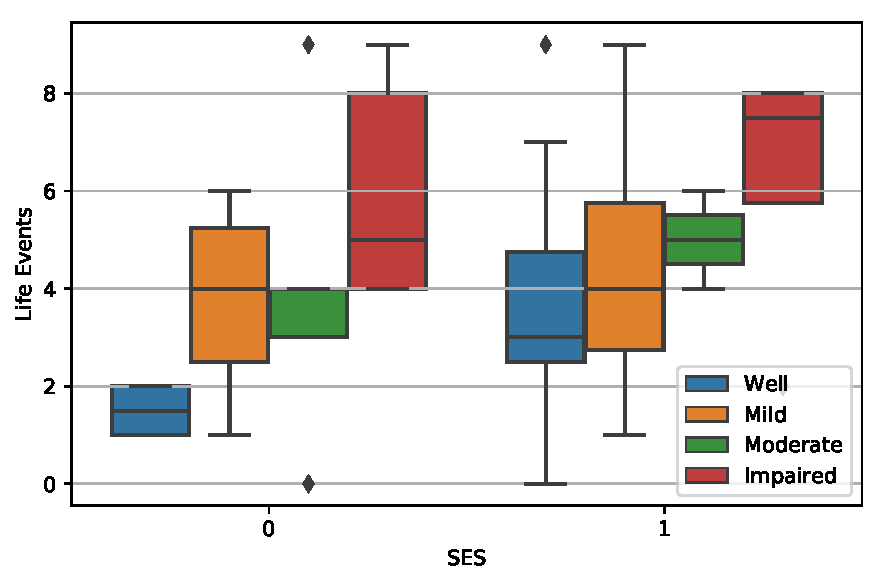
\includegraphics{p6_descriptive.pdf}
    \caption{Boxplots showing the relationship between mental impairment, SES
      and life events.}
    \label{fig:p6_descriptive}
  \end{figure}
  
  \begin{description}
  \item[Solution:] See Figure \ref{fig:p6_descriptive}. Conditioned on SES, the
    expected probability of having a more severe form of mental impairment
    increases with life events.

    The effect of SES on observed mental impairment is more ambiguous. When
    looking at the \texttt{Well} and \texttt{Moderate} levels, it seems that SES
    may have a slight protective effect against mental impairment, for we
    observe many subjects with a high number of life events but no mental
    impairment or less severe impairment. There doesn't seem to be much evidence
    of this phenomenon in the \texttt{Mild} level. Ultimately, there's probably
    not enough data to come to any conclusion about SES.
  \end{description}
\item \label{part:p7} Fit the proportional odds models:
  \begin{align}
    \log\frac{\pi_{ij}}{1 - \pi_{ij}}
    &= \alpha_j^{(0)}
      \label{eqn:p7_model_1} \\
    \log\frac{\pi_{ij}}{1 - \pi_{ij}}
    &= \alpha_j^{(1)} - x_{1i}\beta_1^{(1)}
      \label{eqn:p7_model_2} \\
    \log\frac{\pi_{ij}}{1 - \pi_{ij}}
    &=  \alpha_j^{(2)} - x_{2i}\beta_2^{(2)}
      \label{eqn:p7_model_3} \\
    \log\frac{\pi_{ij}}{1 - \pi_{ij}}
    &= \alpha_j^{(12)} - x_{1i}\beta_1^{(12)} - x_{2i}\beta_2^{(12)}.
      \label{eqn:p7_model_4}
  \end{align}
  Compare models using likelihood ratio statistics, and summarize the
  association between mental impairment, SES and life events, using your favored
  model.

  % latex table generated in R 3.5.1 by xtable 1.8-3 package
% Sun Nov 25 09:16:24 2018
\begin{table}[ht]
\centering
\begin{tabular}{rrrrrrr}
  \toprule
 & $\alpha_0$ & $\alpha_1$ & $\alpha_2$ & $\beta_1$ & $\beta_2$ & Log-likelihood \\ 
  \midrule
Equation \ref{eqn:p7_model_1} & -0.85 & 0.41 & 1.24 & 0.00 & 0.00 & -54.52 \\ 
  Equation \ref{eqn:p7_model_2} & -1.36 & -0.04 & 0.83 & -0.86 & 0.00 & -53.44 \\ 
  Equation \ref{eqn:p7_model_3} & 0.26 & 1.66 & 2.59 & 0.00 & 0.29 & -51.26 \\ 
  Equation \ref{eqn:p7_model_4} & -0.28 & 1.21 & 2.21 & -1.11 & 0.32 & -49.55 \\ 
   \bottomrule
\end{tabular}
\caption{Results of fitting various models corresponding to each equation.} 
\label{tab:p7_model_summary}
\end{table}

  
  \begin{description}
  \item[Solution:] The results of fitting the models can be seen in Table
    \ref{tab:p7_model_summary}. The coefficient estimates agree with what we saw
    in Figure \ref{fig:p6_descriptive} and the discussion in the solution of
    Part \ref{part:p6}: positive $\beta_2$ indicate that observed severity of
    mental impairment increases with life events, and negative $\beta_1$
    indicate that SES lessens the observed severity of mental impairment.

    Wilks' theorem tells us how to compute a test statistic for a log-likelihood
    ratio test:
    \begin{equation}
      D = 2\left(
        l\left(\bm\alpha^{(p)}, \bm\beta^{(p)}\right) -
        l\left(\bm\alpha^{(q)}, \bm\beta^{(q)}\right)        
      \right) \xrightarrow{\mathcal{D}} \chi^2_{p - q},
      \label{eqn:p7_deviance}
    \end{equation}
    where $p > q$ and $\bm\beta^{(p)}$ and $\bm\beta^{(q)}$ each have
    dimensionality $p$ and $q$, respectively. That is, the deviance converges
    asymptotically to a chi-squared distribution with degrees of $p-q$.

    The test statistic in Equation \ref{eqn:p7_deviance} can be computed for
    various pairs of models with the last column of Table
    \ref{tab:p7_model_summary} when one of the models in the pair contains a
    superset of the parameters in the null model.
  \end{description}
\item Provide a plot of fitted probabilities under the model in Equation
  \ref{eqn:p7_model_4}, as a function of $x_1$ and $x_2$.

  \begin{figure}
    \centering
    \caption{Fitted probabilities of mental impairment levels using the model
      described in Equation \ref{eqn:p7_model_4}}
    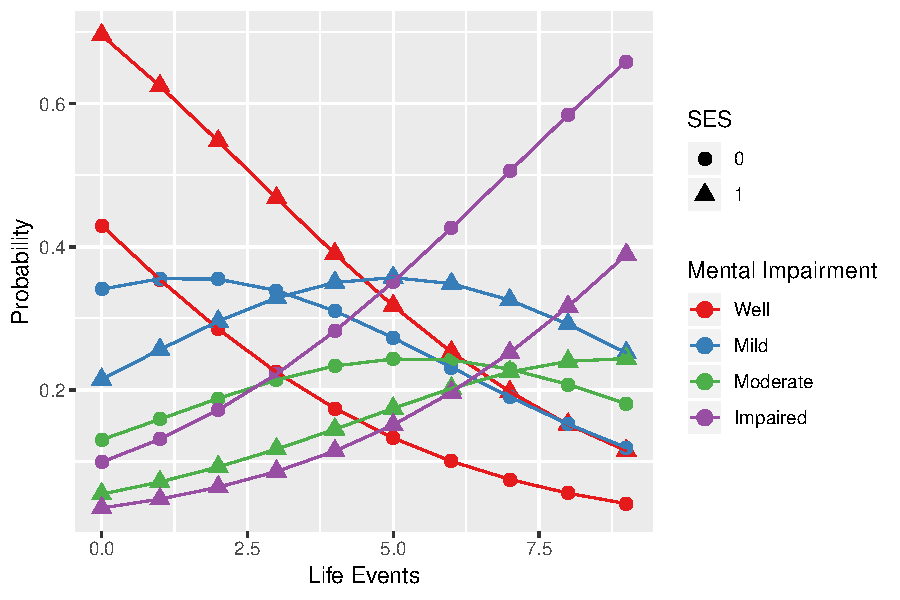
\includegraphics{p8_fitted_probabilities.pdf}
    \label{fig:p8_fitted_probabilities}
  \end{figure}
  
  \begin{description}
  \item[Solution:] See Figure \ref{fig:p8_fitted_probabilities}. As described in
    the solution of Part \ref{part:p7},
  \end{description}
\end{enumerate}

\clearpage

\section*{Appendix}

\subsection*{Code}

Code for the logistic regression model and boxplots can be found in
\href{http://nbviewer.jupyter.org/github/ppham27/stat570/blob/master/hw7/mental_impairment.ipynb}{\texttt{mental\_impairment.ipynb}}. Code
for the proportional odds models and Figure \ref{fig:p8_fitted_probabilities}
can be found in
\href{http://nbviewer.jupyter.org/github/ppham27/stat570/blob/master/hw7/proportional\_odds.ipynb}{\texttt{proportional\_odds.ipynb}}.

\subsection*{Data}

The raw mental impairment data is in Table \ref{tab:p1_data}.

\begin{table}[h]
  \scriptsize
  \centering
  \begin{tabular}{rlrr}
\toprule
 Subject & Mental Impairment &  SES &  Life Events \\
\midrule
       1 &              Well &    1 &            1 \\
       2 &              Well &    1 &            9 \\
       3 &              Well &    1 &            4 \\
       4 &              Well &    1 &            3 \\
       5 &              Well &    0 &            2 \\
       6 &              Well &    1 &            0 \\
       7 &              Well &    0 &            1 \\
       8 &              Well &    1 &            3 \\
       9 &              Well &    1 &            3 \\
      10 &              Well &    1 &            7 \\
      11 &              Well &    0 &            1 \\
      12 &              Well &    0 &            2 \\
      13 &              Mild &    1 &            5 \\
      14 &              Mild &    0 &            6 \\
      15 &              Mild &    1 &            3 \\
      16 &              Mild &    0 &            1 \\
      17 &              Mild &    1 &            8 \\
      18 &              Mild &    1 &            2 \\
      19 &              Mild &    0 &            5 \\
      20 &              Mild &    1 &            5 \\
      21 &              Mild &    1 &            9 \\
      22 &              Mild &    0 &            3 \\
      23 &              Mild &    1 &            3 \\
      24 &              Mild &    1 &            1 \\
      25 &          Moderate &    0 &            0 \\
      26 &          Moderate &    1 &            4 \\
      27 &          Moderate &    0 &            3 \\
      28 &          Moderate &    0 &            9 \\
      29 &          Moderate &    1 &            6 \\
      30 &          Moderate &    0 &            4 \\
      31 &          Moderate &    0 &            3 \\
      32 &          Impaired &    1 &            8 \\
      33 &          Impaired &    1 &            2 \\
      34 &          Impaired &    1 &            7 \\
      35 &          Impaired &    0 &            5 \\
      36 &          Impaired &    0 &            4 \\
      37 &          Impaired &    0 &            4 \\
      38 &          Impaired &    1 &            8 \\
      39 &          Impaired &    0 &            8 \\
      40 &          Impaired &    0 &            9 \\
\bottomrule
\end{tabular}

  \caption{Data on mental impairment, socioeconomic status (SES) and life
    events, for 40 subjects.}
  \label{tab:p1_data}
\end{table}

\end{document}
